\documentclass[12pt,a4paper]{report}
\usepackage[latin1]{inputenc}
\usepackage{amsmath}
\usepackage{amsfonts}
\usepackage{subfigure}
\usepackage{amssymb}
\usepackage[pdftex]{graphicx}
\begin{document}
\noindent
{\bf The Story} \\
A metric learning-like framework is proposed for unsupervised training of neural networks. As demonstrated in algorithms such as DrLIM, ISOMAP and others, learning a metric can implicitly lead to a representation in which the underlying latent variables are disentangled or linearized. However the approach relies on an oracle to provide semantically meaningful similarity relationships. Temporal coherence can be exploited to provide similarity relationships needed to learn a semantically meaningful metric: temporally neighboring frames in a video are likely to be semantic neighbors. The objective thus becomes to extract slowly varying temporal features which closely resembles slow feature analysis (SFA). However the proposed algorithm differes from SFA in two important ways. Firstly, the slow features need not be linear functions of the input. Secondly, we explicitly enforce that the feature representation be information preserving by minimizing reconstruction error. The last requirement naturally leads to a Siamese auto-encoder like architecture which lead to the name Temporal Auto-Encoder (TAE). \\ \\

\noindent 
{\bf Motivation: Metric Learning as Unsupervised Feature Learning} 
Toy examples when DrLIM learns independent factors of variation:  
\begin{center}
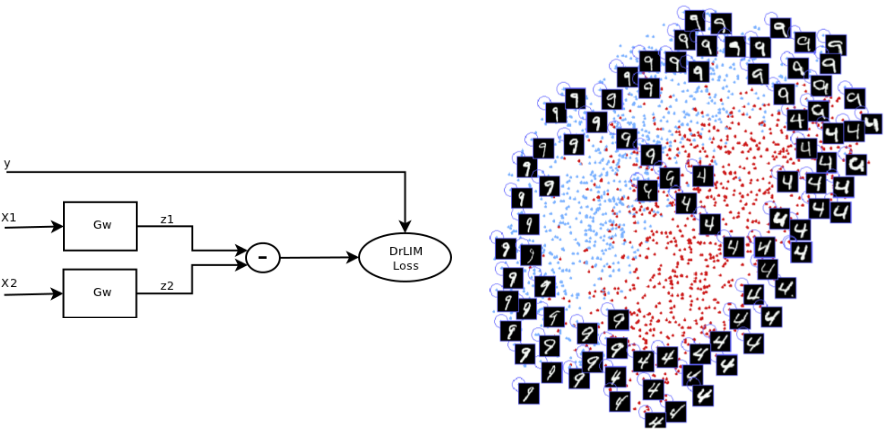
\includegraphics[scale=0.4]{drlim_mnist.png}
\end{center} 
\newpage
Temporal toy data: rotating airplane 
\begin{center}
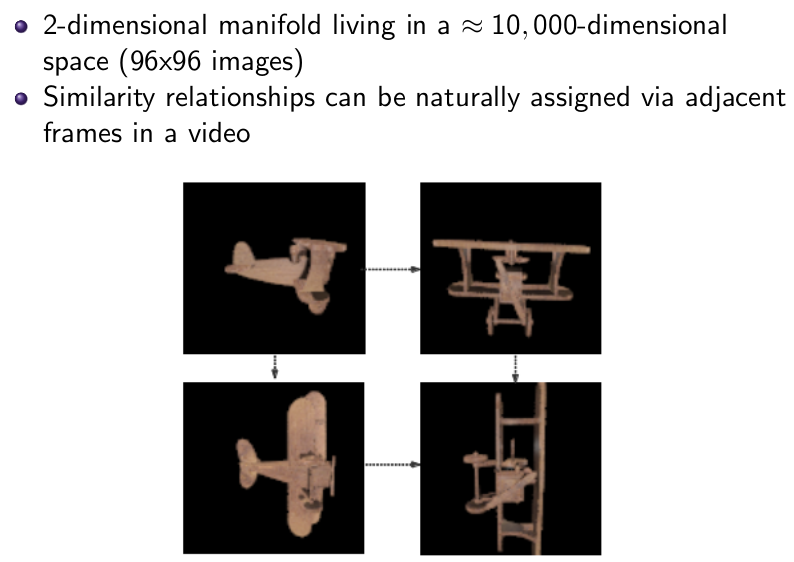
\includegraphics[scale=0.4]{drlim_data.png}
\end{center} 
Learns to implicitly extract angles of rotation, i.e. true latent variables.  
\begin{center}
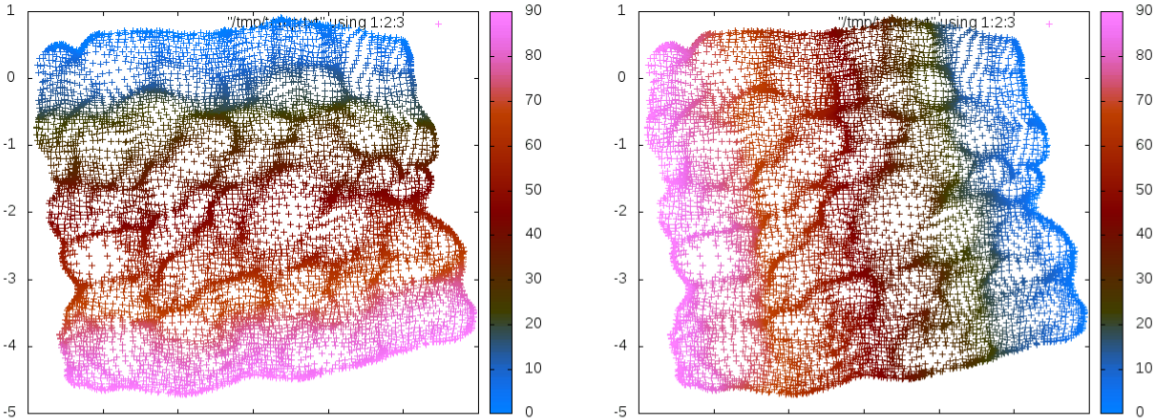
\includegraphics[scale=0.3]{drlim_result.png}
\end{center}
\newpage 

{\bf Summary of Results} \\ \\
\underline{Sparse-Transition Features} 
\begin{center} 
$L = \sum_{i=1} ^2 \frac{1}{2}\|x_i - W_d~z_i\|^2 +\alpha|z_1 - z_2|$ where $z_i = ReLU(W_e~x_i)$ 
\end{center} 
The resulting basis found using slowness (or sparse-transitions since $L_1$ is used) alone is similar, but not identical to those obtained by a sparse auto-encoder.    
\begin{center}
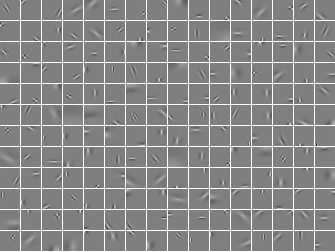
\includegraphics[scale=0.5]{SF.png}
\end{center} 
\underline{Sparse/Slow Pooled Features} 
\begin{center}
 $L = \sum_{i=1} ^2 \left(\frac{1}{2}\|x_i - W_d~h_i)\|^2 +\alpha|h_i|\right) + \beta|z_1 - z_2|$ 
\end{center}   
Where, $h_i = ReLU(W_ex_i)$ and $z_i = pool(h)$. That is $pool()$ is a pooling operator which includes pooling across features as well as neighboring spatial locations in the convolutional setting. $W_e$ and $W_d$ are learned linear operators which may be convolutional. Thus the feed-forward mapping from the input $x$ to the feature space $z$ is given by $z = pool(ReLU(W_e~x))$ which corresponds to a single stage in the most widely used convolutional networks if $W_e$ is a convolutional operator.  
\begin{figure}
\centering
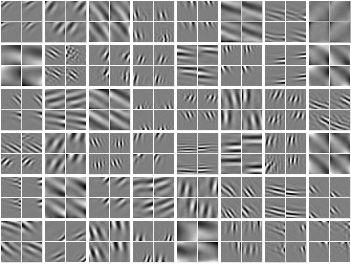
\includegraphics[scale=0.5]{SF_pool_SF.png}
\caption{$L_2$ pooled fully connected sparse/slow features}
\end{figure}  
\newpage

\underline{Sparse/Slow Pooled Convolutional Features} \\

\begin{figure}
\centering
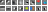
\includegraphics[scale=5]{L2_f2s1.png}
\caption{$L_2$ pooled 2-pooling }
\end{figure} 

\end{document} 